\subsection{Moduł aministracyjny}

\begin{itemize}
	\item Wymagania funkcjonalne dotyczące modułu administracyjnego zostały opisane w sekcji 1.3.1. Pierwsze pięć z nich dotyczą czynności związanych z autoryzacją administratora. Użytkownikowi posiadającemu status administratora, aplikacja umożliwia logowanie, resetowanie hasła w przypadku jego utraty, zmianę hasła i adresu email, gdy administrator jest już zalogowany, oraz wylogowanie. Widoki umożliwiające dokonanie ww. działań zostały przedstawione poniżej. 

\vspace{0,5cm}
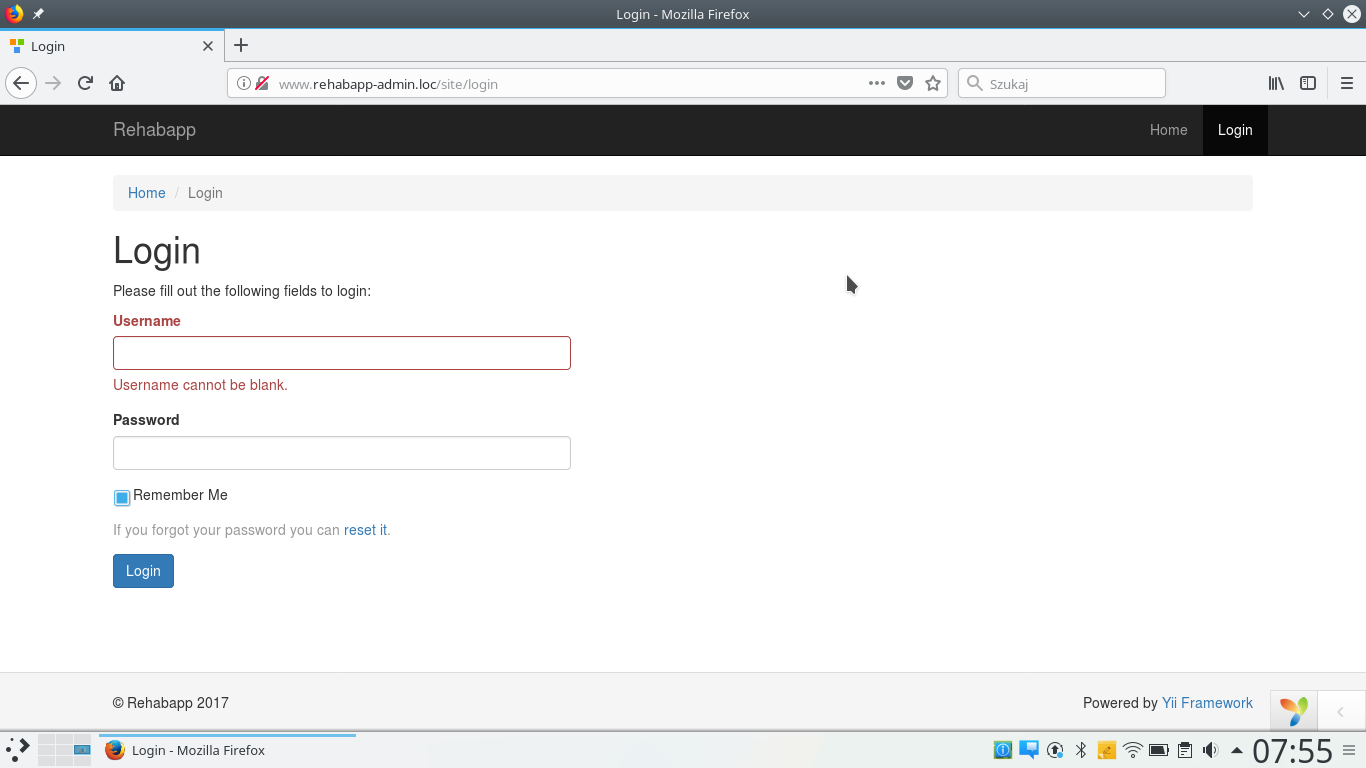
\includegraphics[scale=0.4]{obraz/1.png}
%\begin{center}{\scriptsize Rysunek 1: Diagram przypadków użycia.}\end{center}
\vspace{0,5cm}

\vspace{0,5cm}
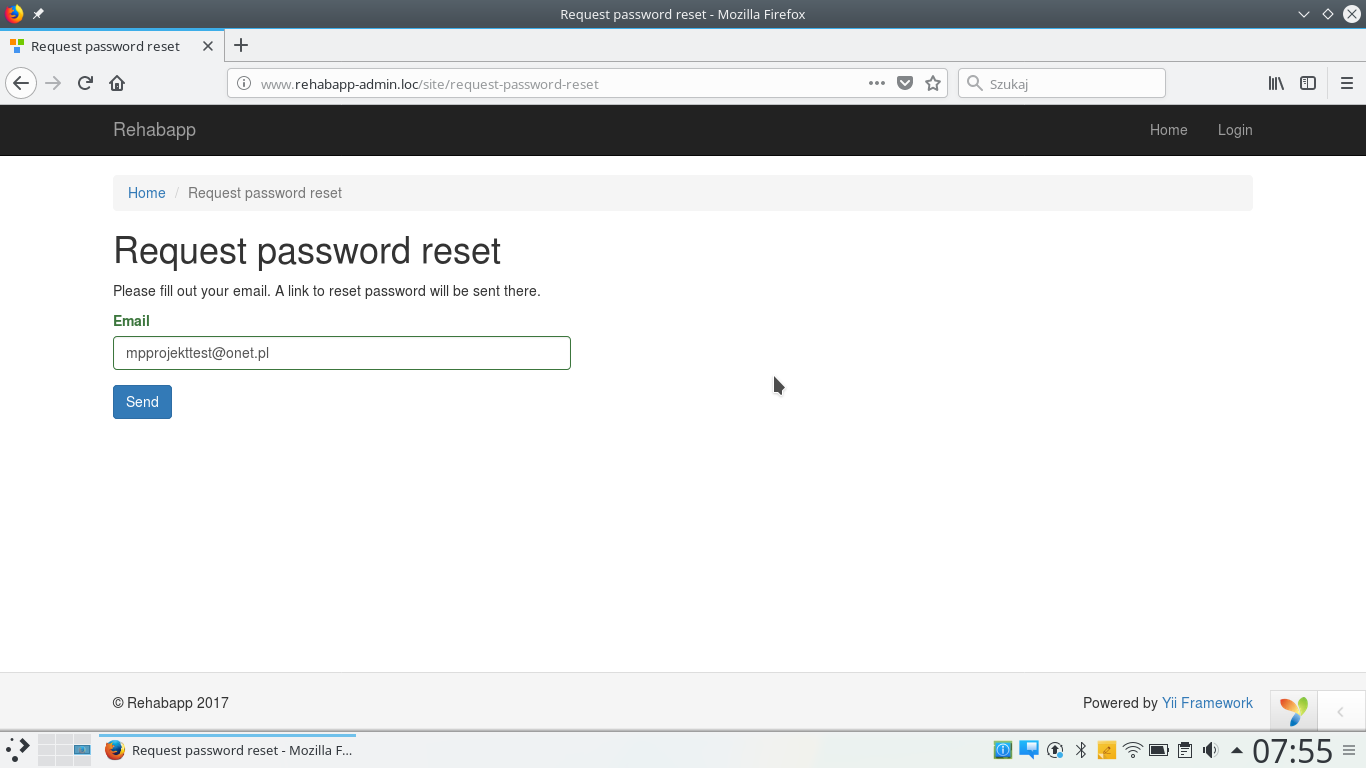
\includegraphics[scale=0.4]{obraz/2.png}
%\begin{center}{\scriptsize Rysunek 1: Diagram przypadków użycia.}\end{center}
\vspace{0,5cm}

\vspace{0,5cm}
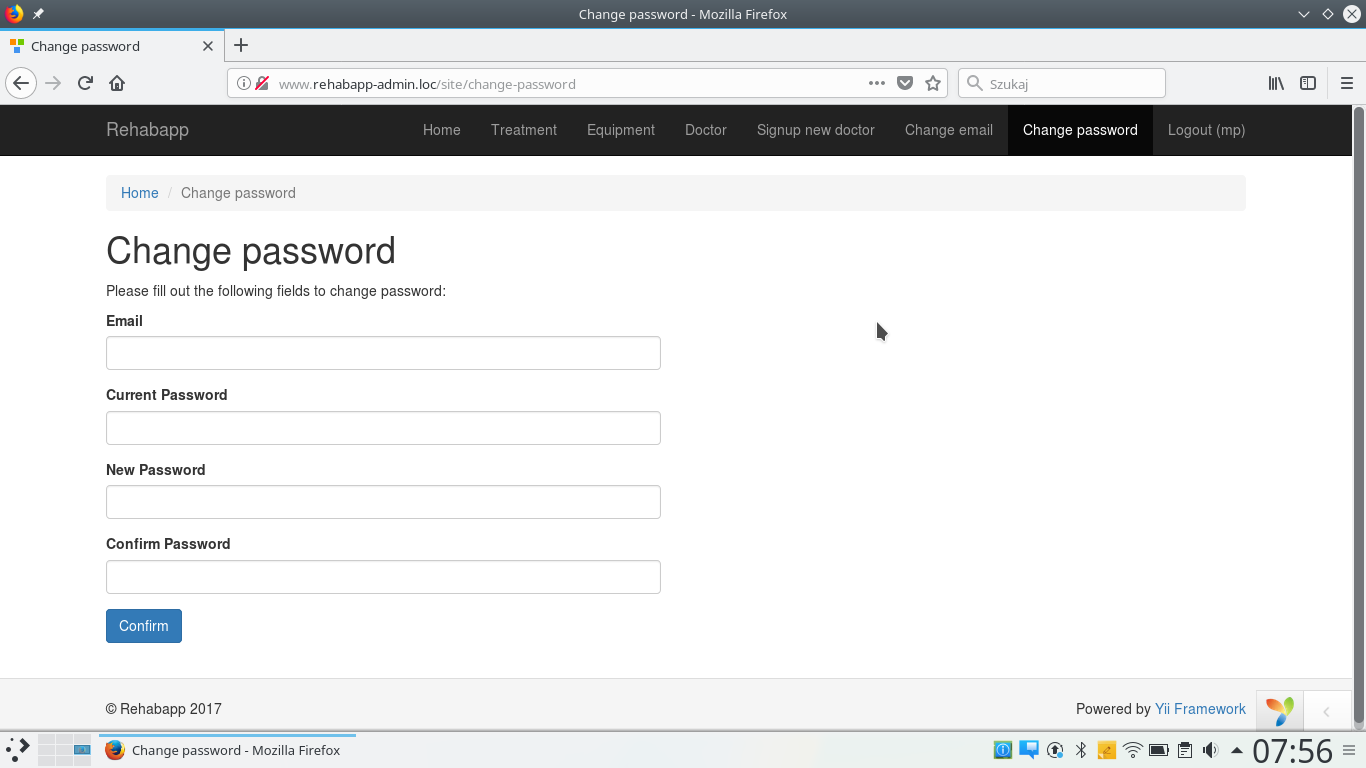
\includegraphics[scale=0.4]{obraz/3.png}
%\begin{center}{\scriptsize Rysunek 1: Diagram przypadków użycia.}\end{center}
\vspace{0,5cm}

\vspace{0,5cm}
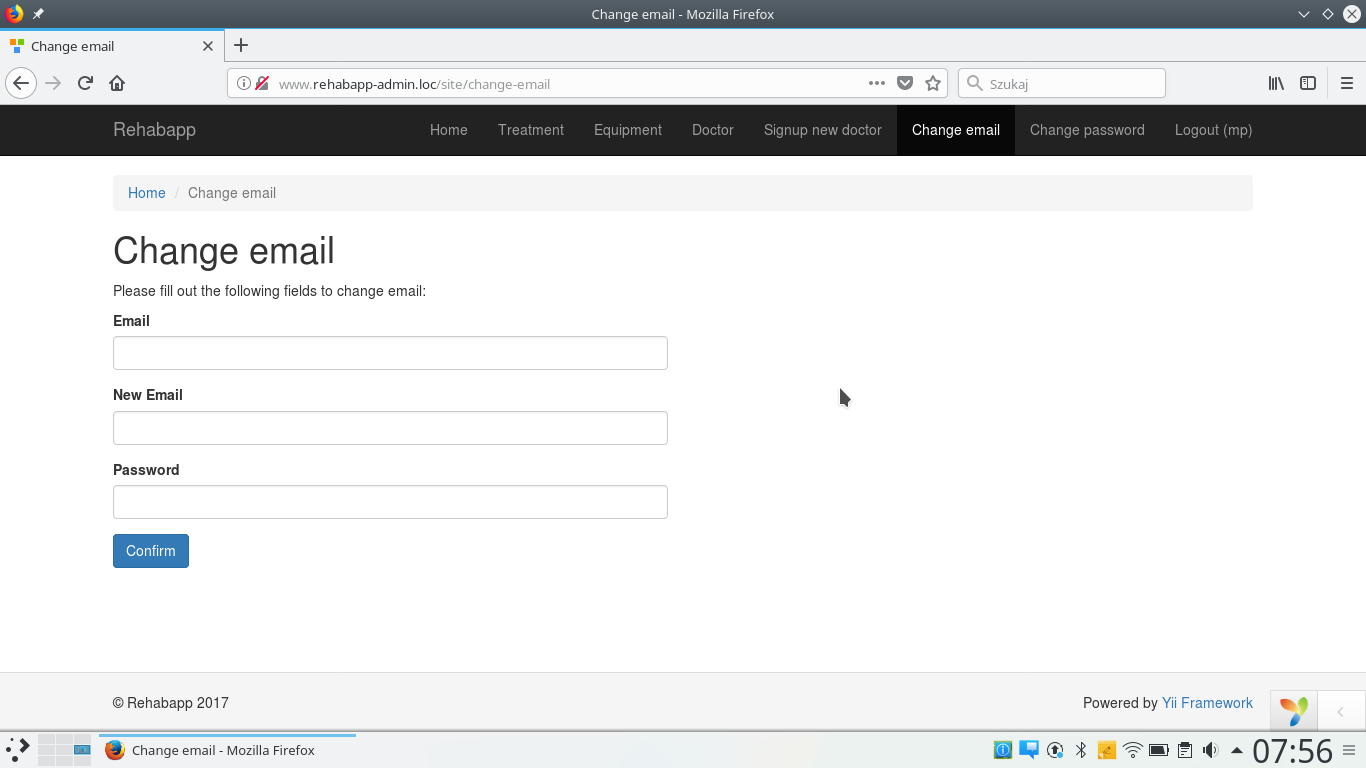
\includegraphics[scale=0.4]{obraz/4.png}
%\begin{center}{\scriptsize Rysunek 1: Diagram przypadków użycia.}\end{center}
\vspace{0,5cm}
\newpage
	\item Kolejne 5 wymagań dotyczyło zarządzania zasobami placówki. System umożliwia dodawanie, edycję, usuwanie, wyświetlanie szczegółów dotyczących sprzętu oraz listę wszystkich zapisanych w bazie zasobów.
	
\vspace{0,5cm}
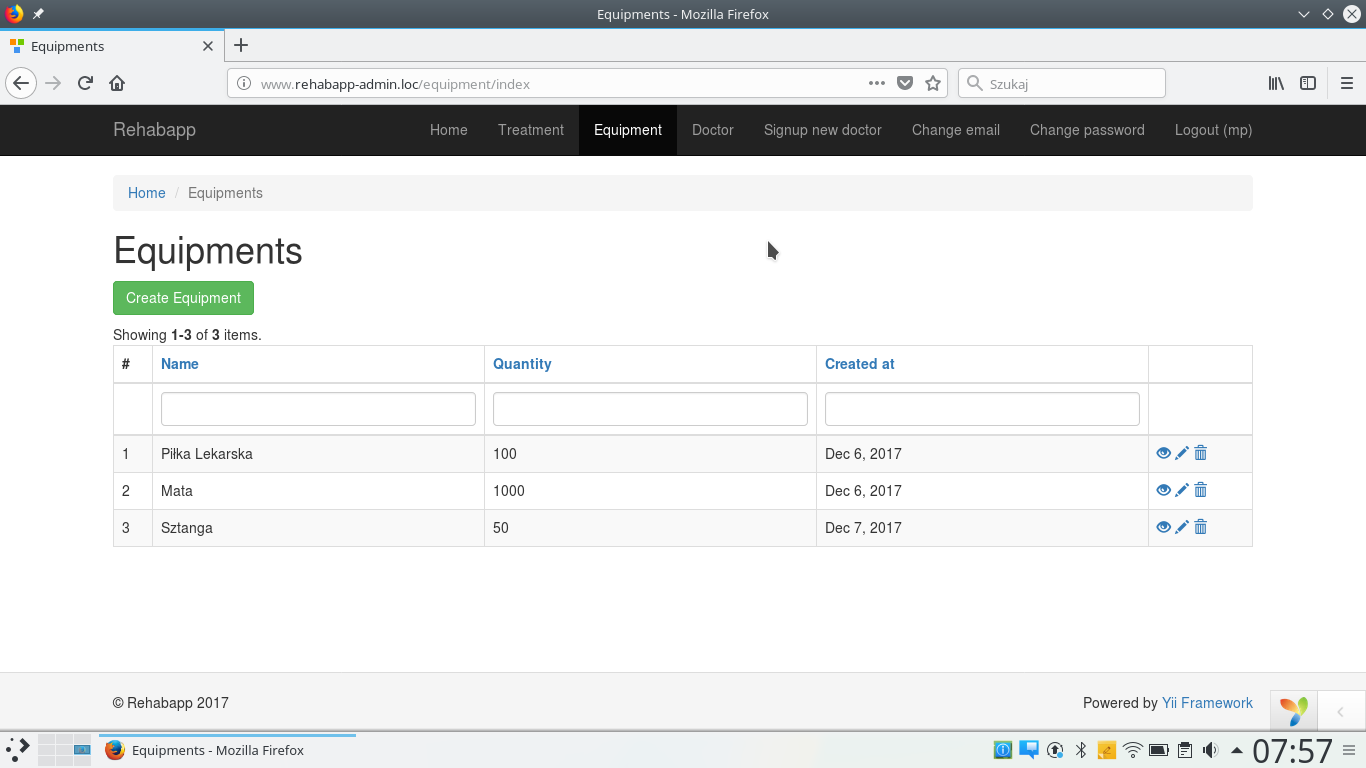
\includegraphics[scale=0.4]{obraz/5.png}
%\begin{center}{\scriptsize Rysunek 1: Diagram przypadków użycia.}\end{center}
\vspace{0,5cm}

\vspace{0,5cm}
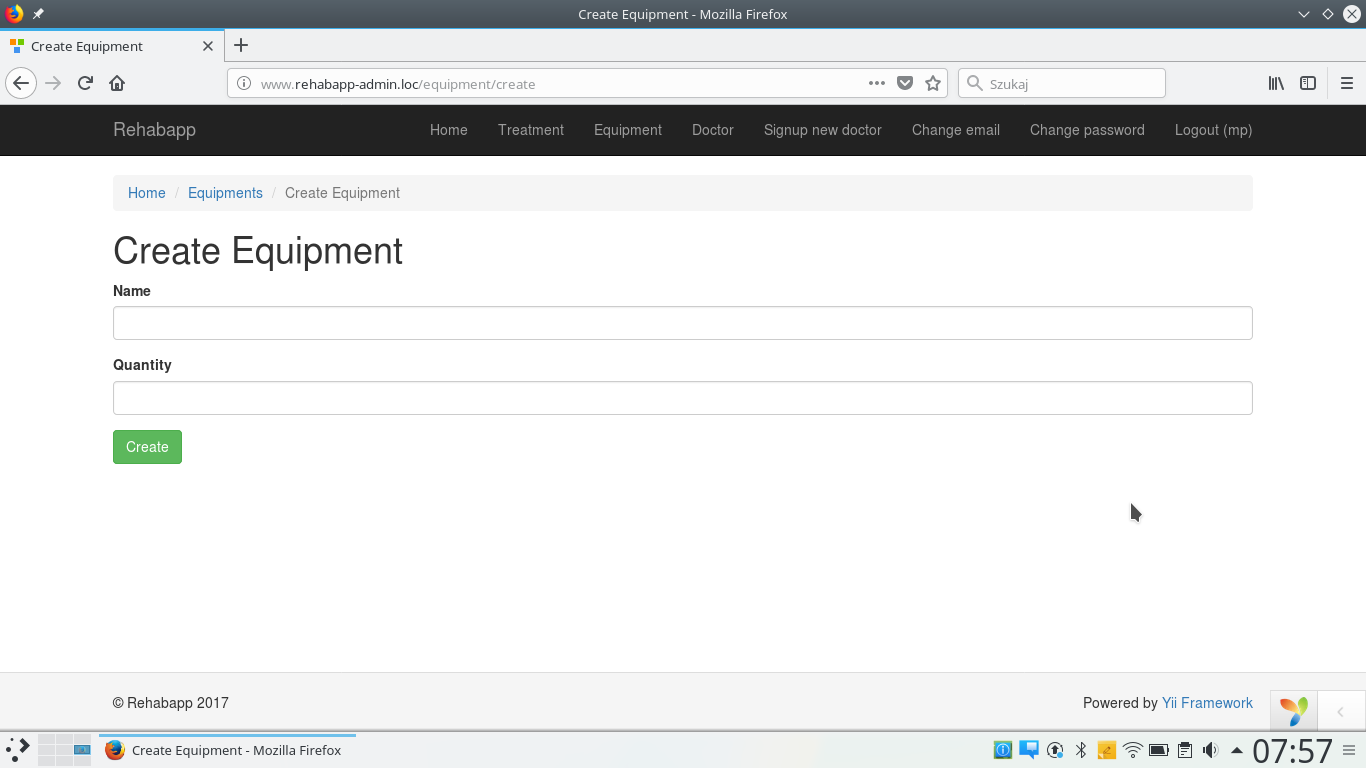
\includegraphics[scale=0.4]{obraz/6.png}
%\begin{center}{\scriptsize Rysunek 1: Diagram przypadków użycia.}\end{center}
\vspace{0,5cm}

\vspace{0,5cm}
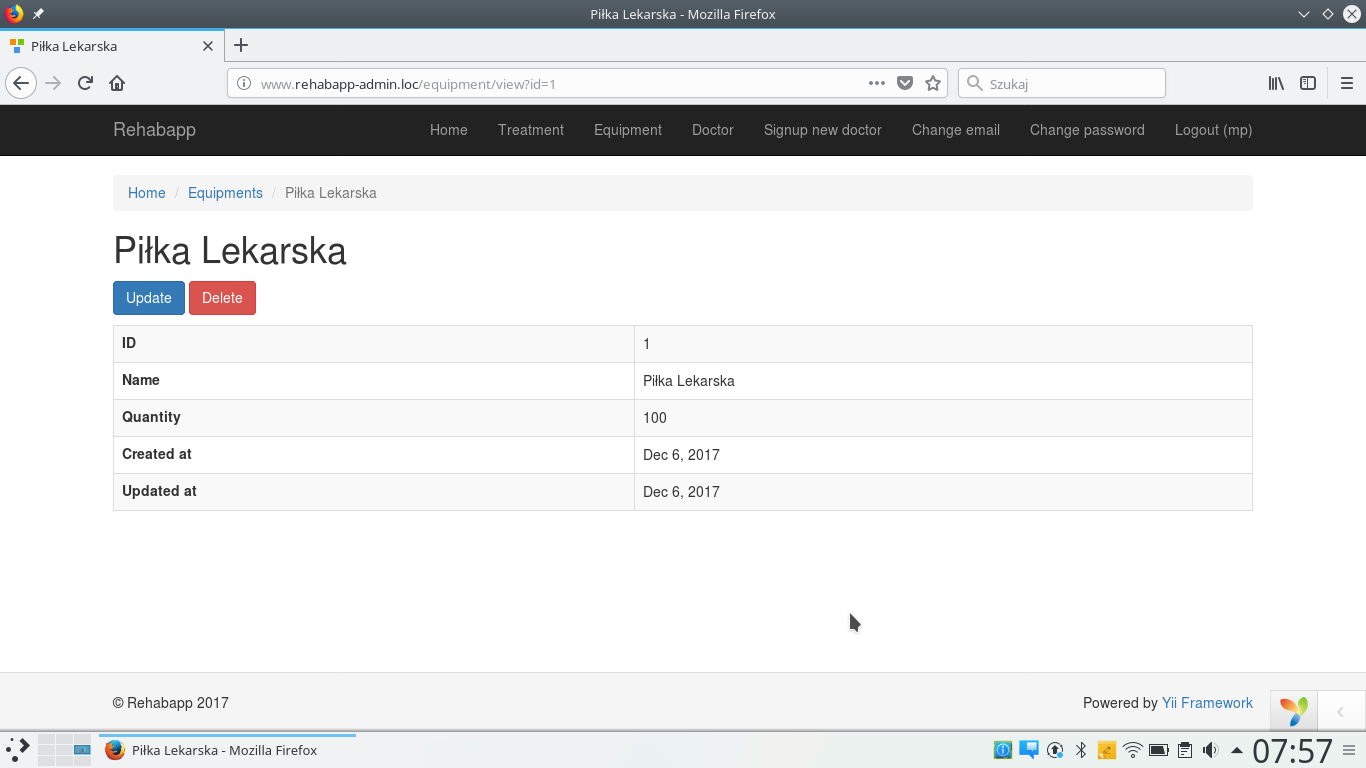
\includegraphics[scale=0.4]{obraz/7.png}
%\begin{center}{\scriptsize Rysunek 1: Diagram przypadków użycia.}\end{center}
\vspace{0,5cm}

\vspace{0,5cm}
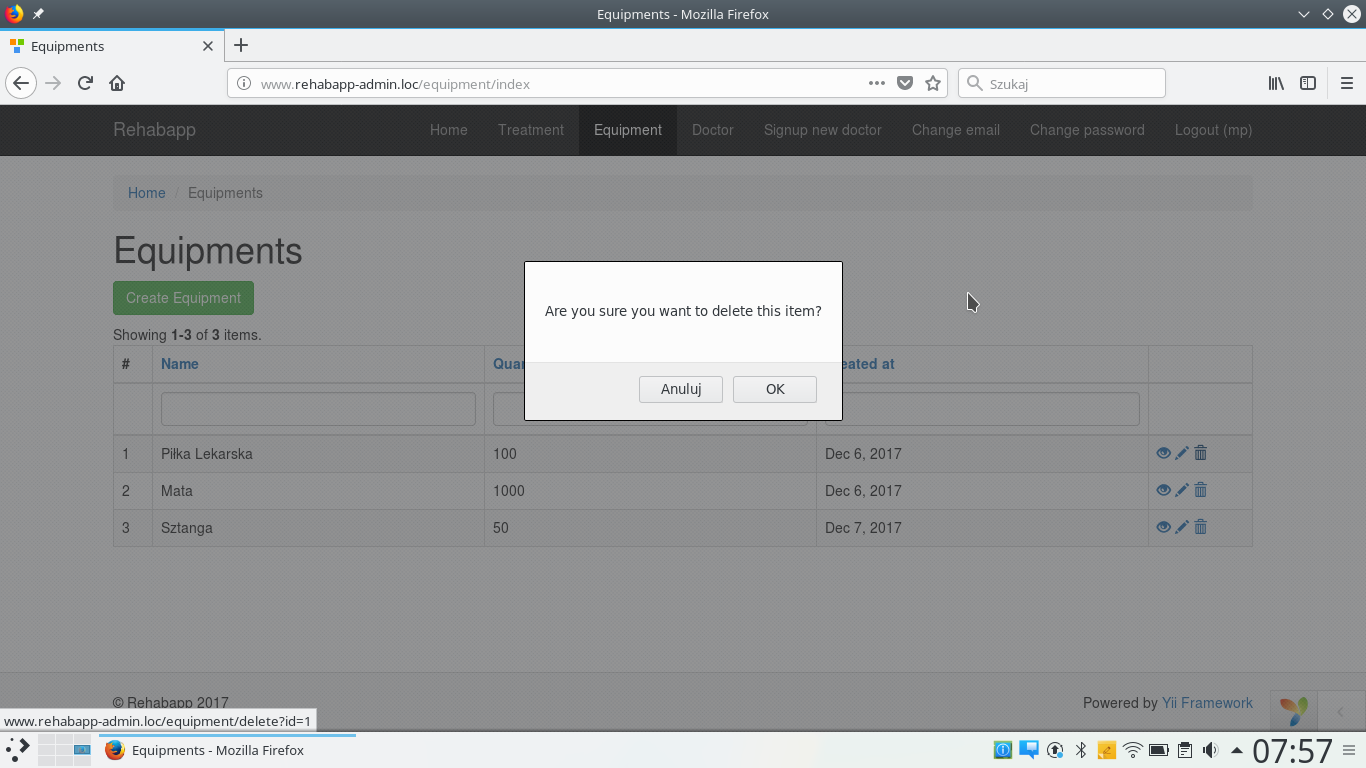
\includegraphics[scale=0.4]{obraz/8.png}
%\begin{center}{\scriptsize Rysunek 1: Diagram przypadków użycia.}\end{center}
\vspace{0,5cm}
\newpage
	\item Uprawnienia administratora umożliwiają również zarządzanie zabiegami. Wszystkie funkcjonalności dotyczące zabiegów w systemie zostały zaimplementowane zgodnie z wymaganiami o numerach od 11 do 15.
	
	
\vspace{0,5cm}
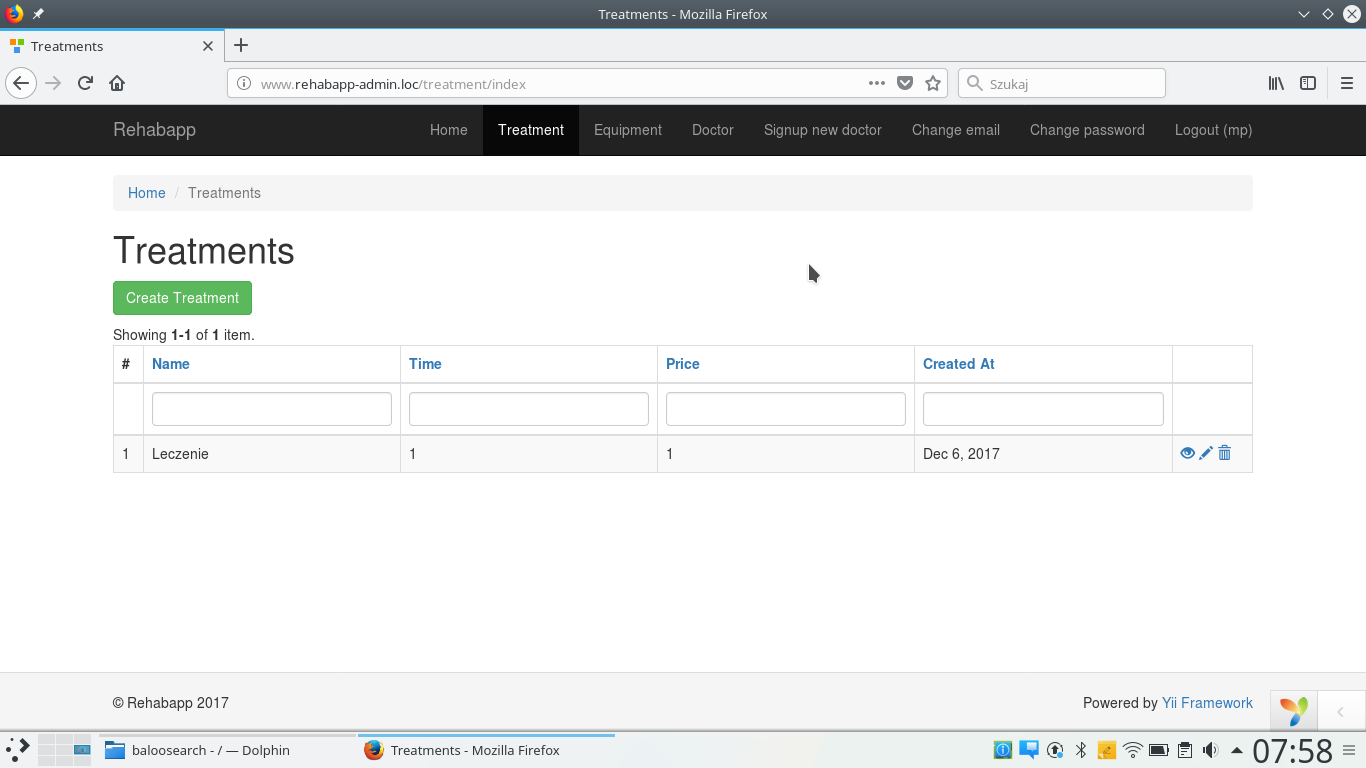
\includegraphics[scale=0.4]{obraz/9.png}
%\begin{center}{\scriptsize Rysunek 1: Diagram przypadków użycia.}\end{center}
\vspace{0,5cm}

\vspace{0,5cm}
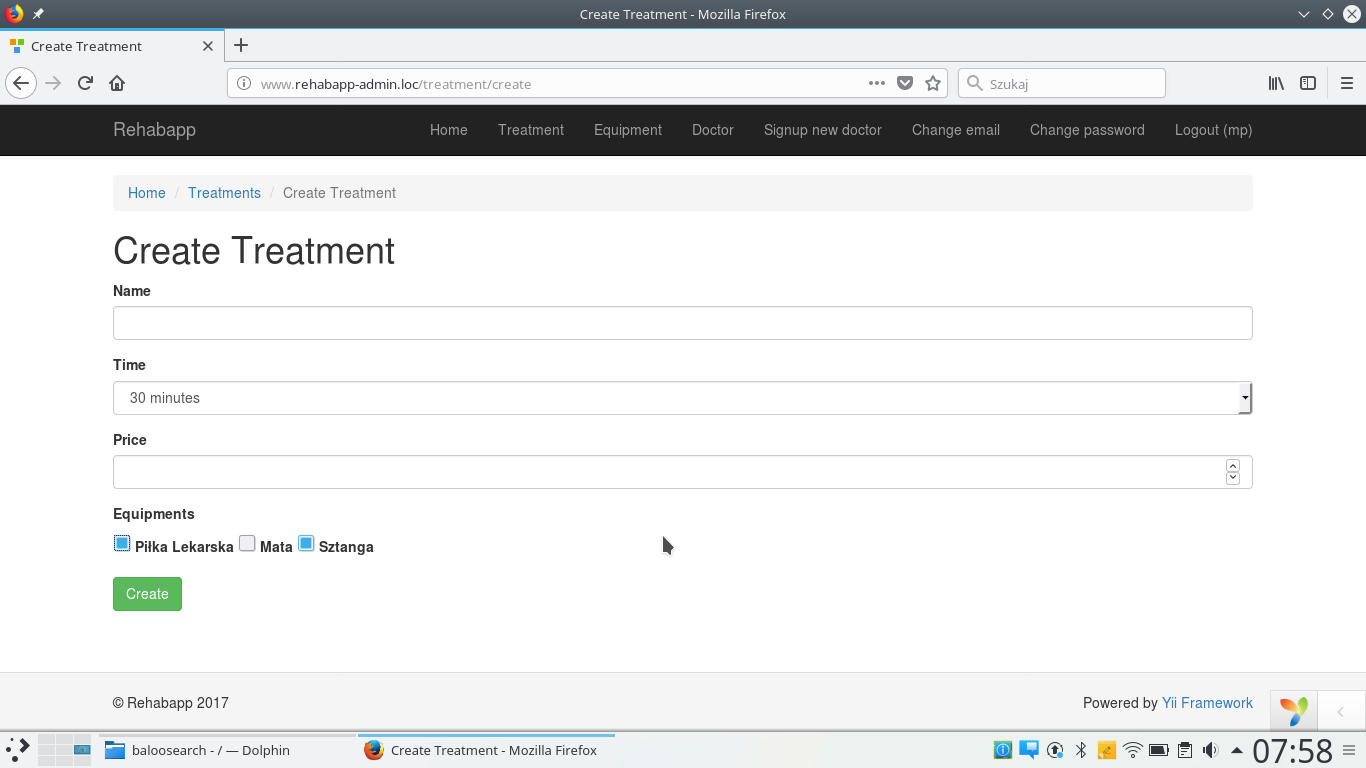
\includegraphics[scale=0.4]{obraz/10.png}
%\begin{center}{\scriptsize Rysunek 1: Diagram przypadków użycia.}\end{center}
\vspace{0,5cm}

\vspace{0,5cm}
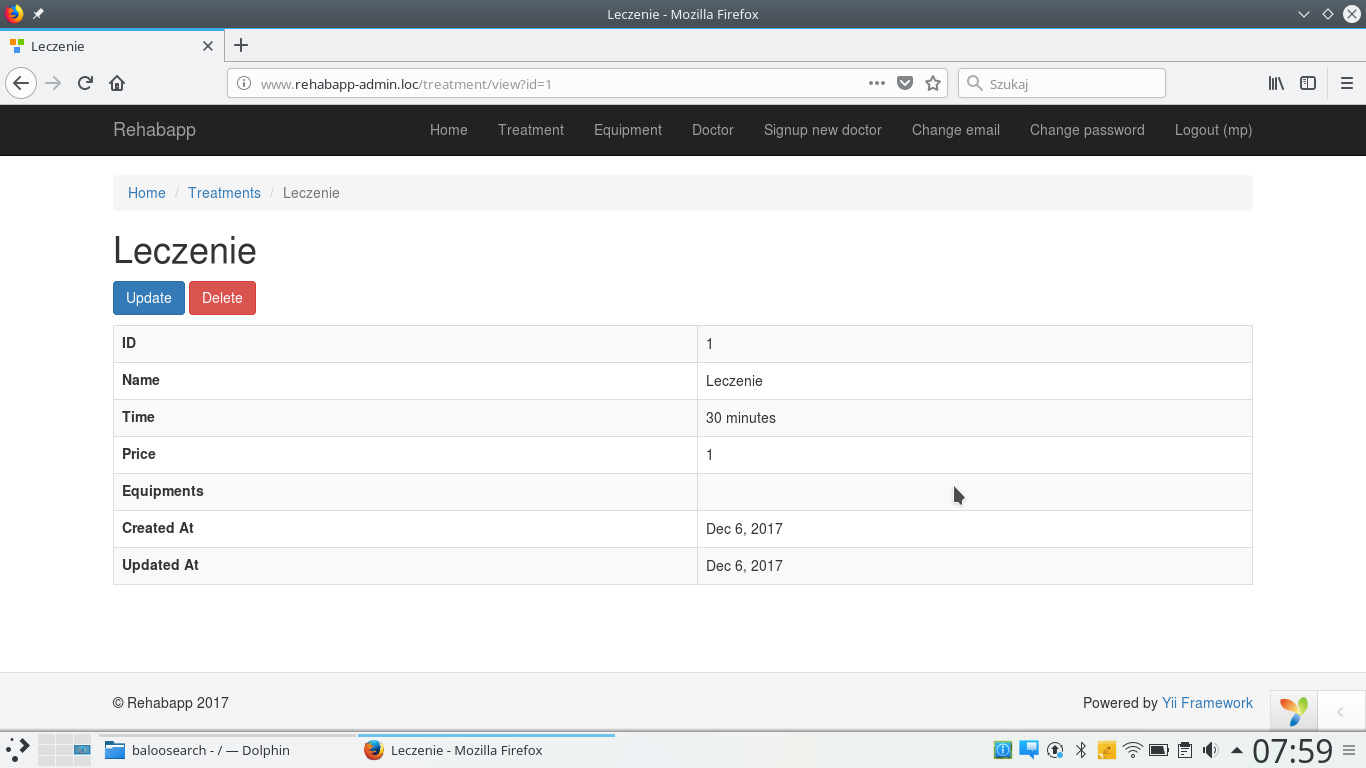
\includegraphics[scale=0.4]{obraz/11.png}
%\begin{center}{\scriptsize Rysunek 1: Diagram przypadków użycia.}\end{center}
\vspace{0,5cm}

\vspace{0,5cm}
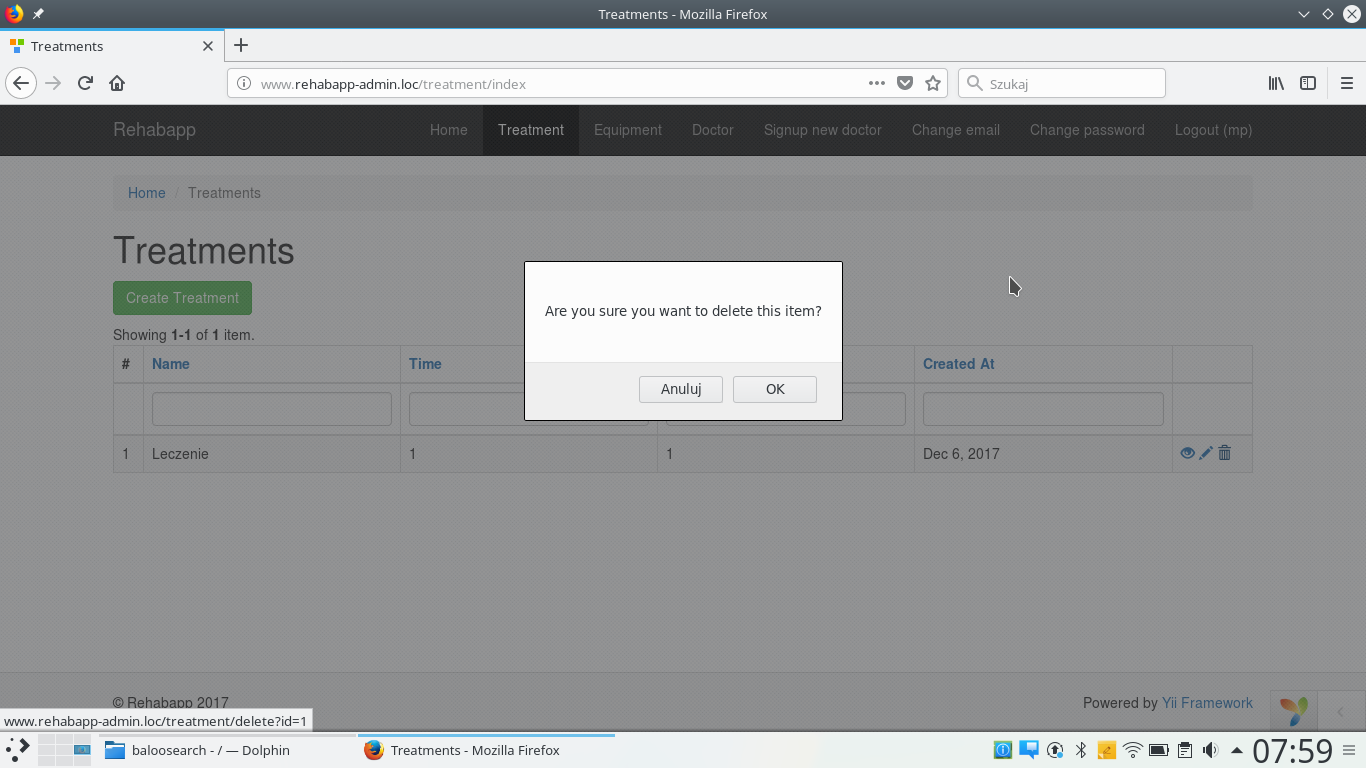
\includegraphics[scale=0.4]{obraz/12.png}
%\begin{center}{\scriptsize Rysunek 1: Diagram przypadków użycia.}\end{center}
\vspace{0,5cm}
\newpage
	\item Administrator ma również możliwość zarządzania (zgodnie z wymaganiami od 16 do 22) inną grupą użytkowników systemów, jaką są lekarze. Czynności tego dotyczące to dodawanie, edycja i usuwanie lekarzy, wyświetlanie listy wszystkich lekarzy pracujących w placówce, wyświetlanie szczegółów dotyczących konkretnego lekarza, a także zmiana hasła i dodawanie terminów wizyt lekarzowi.
	
	
\vspace{0,5cm}
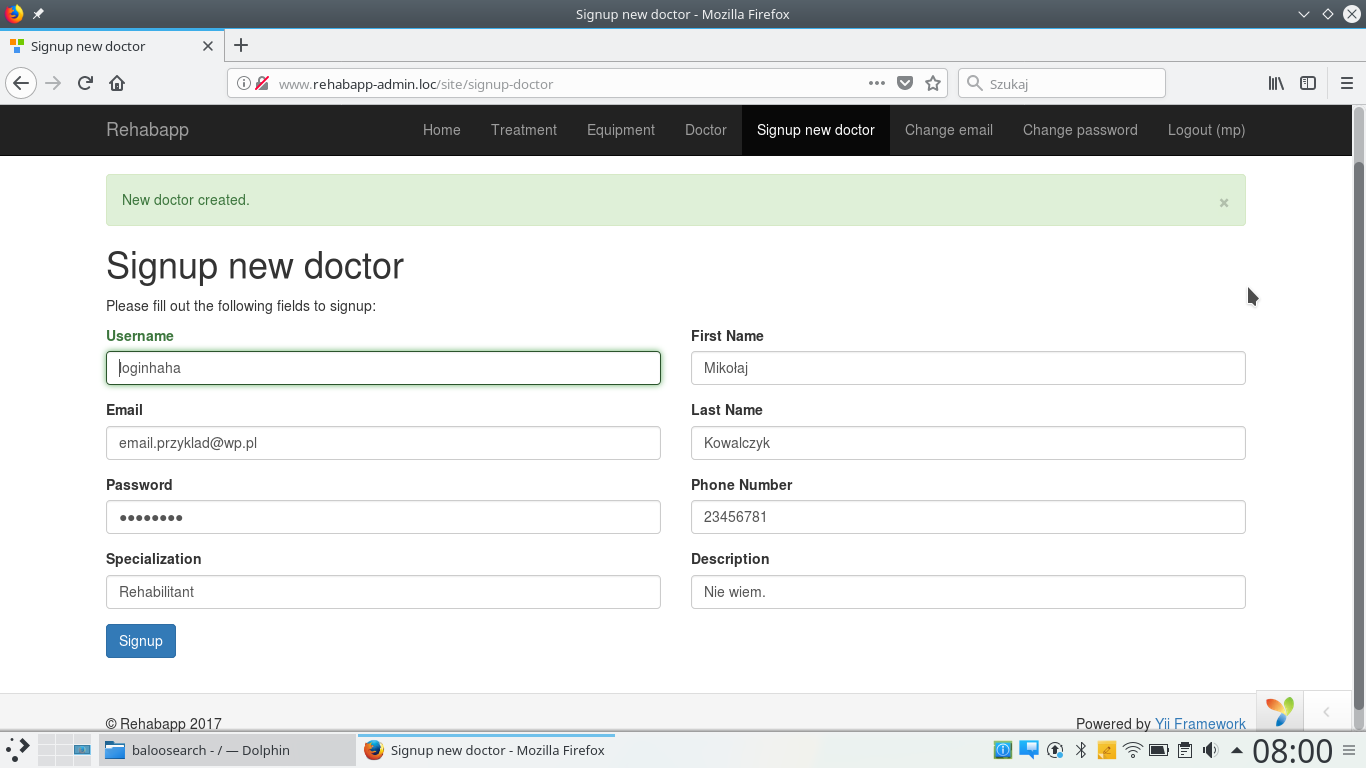
\includegraphics[scale=0.4]{obraz/13.png}
%\begin{center}{\scriptsize Rysunek 1: Diagram przypadków użycia.}\end{center}
\vspace{0,5cm}

\vspace{0,5cm}
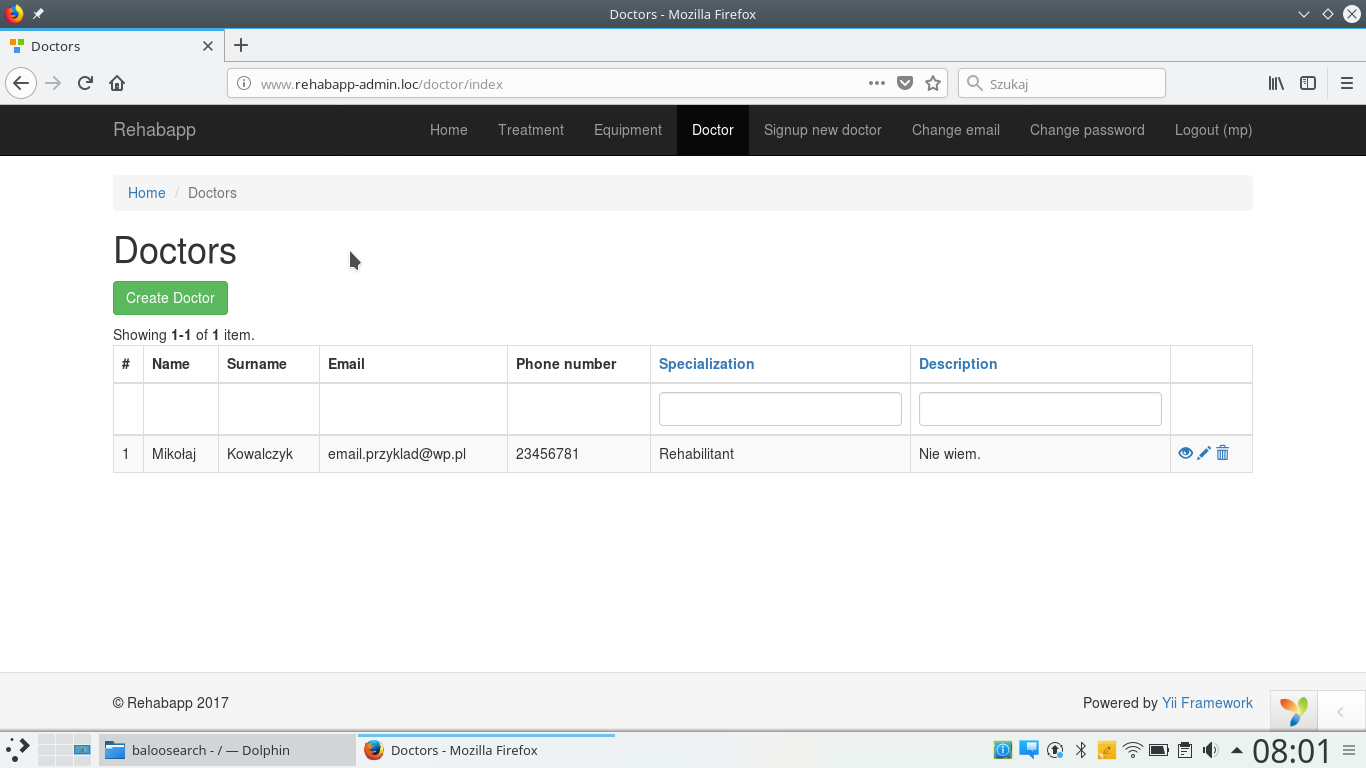
\includegraphics[scale=0.4]{obraz/14.png}
%\begin{center}{\scriptsize Rysunek 1: Diagram przypadków użycia.}\end{center}
\vspace{0,5cm}

\vspace{0,5cm}
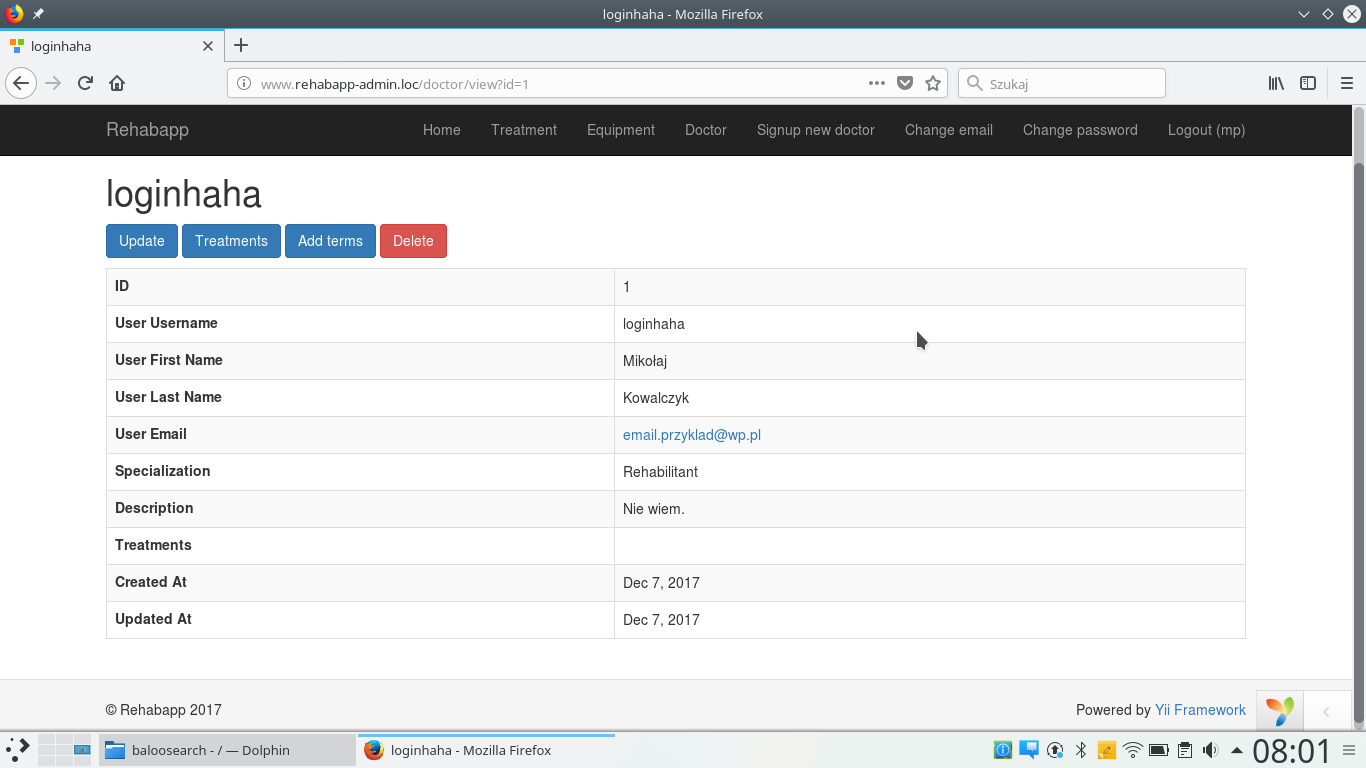
\includegraphics[scale=0.4]{obraz/15.png}
%\begin{center}{\scriptsize Rysunek 1: Diagram przypadków użycia.}\end{center}
\vspace{0,5cm}

\vspace{0,5cm}
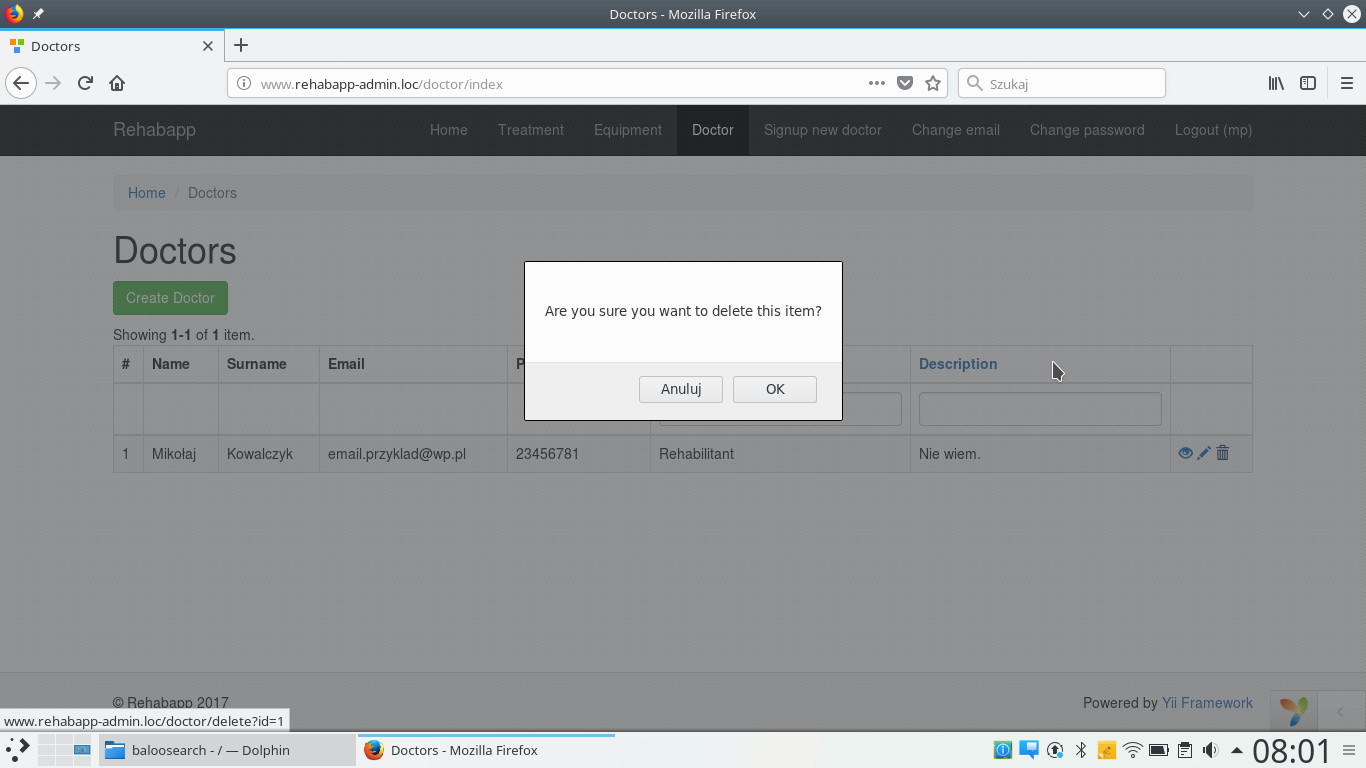
\includegraphics[scale=0.4]{obraz/16.png}
%\begin{center}{\scriptsize Rysunek 1: Diagram przypadków użycia.}\end{center}
\vspace{0,5cm}
	


\end{itemize}
\newpage
